\documentclass[11pt]{beamer}\usepackage[]{graphicx}\usepackage[]{color}
% maxwidth is the original width if it is less than linewidth
% otherwise use linewidth (to make sure the graphics do not exceed the margin)
\makeatletter
\def\maxwidth{ %
  \ifdim\Gin@nat@width>\linewidth
    \linewidth
  \else
    \Gin@nat@width
  \fi
}
\makeatother

\definecolor{fgcolor}{rgb}{0.345, 0.345, 0.345}
\newcommand{\hlnum}[1]{\textcolor[rgb]{0.686,0.059,0.569}{#1}}%
\newcommand{\hlstr}[1]{\textcolor[rgb]{0.192,0.494,0.8}{#1}}%
\newcommand{\hlcom}[1]{\textcolor[rgb]{0.678,0.584,0.686}{\textit{#1}}}%
\newcommand{\hlopt}[1]{\textcolor[rgb]{0,0,0}{#1}}%
\newcommand{\hlstd}[1]{\textcolor[rgb]{0.345,0.345,0.345}{#1}}%
\newcommand{\hlkwa}[1]{\textcolor[rgb]{0.161,0.373,0.58}{\textbf{#1}}}%
\newcommand{\hlkwb}[1]{\textcolor[rgb]{0.69,0.353,0.396}{#1}}%
\newcommand{\hlkwc}[1]{\textcolor[rgb]{0.333,0.667,0.333}{#1}}%
\newcommand{\hlkwd}[1]{\textcolor[rgb]{0.737,0.353,0.396}{\textbf{#1}}}%
\let\hlipl\hlkwb

\usepackage{framed}
\makeatletter
\newenvironment{kframe}{%
 \def\at@end@of@kframe{}%
 \ifinner\ifhmode%
  \def\at@end@of@kframe{\end{minipage}}%
  \begin{minipage}{\columnwidth}%
 \fi\fi%
 \def\FrameCommand##1{\hskip\@totalleftmargin \hskip-\fboxsep
 \colorbox{shadecolor}{##1}\hskip-\fboxsep
     % There is no \\@totalrightmargin, so:
     \hskip-\linewidth \hskip-\@totalleftmargin \hskip\columnwidth}%
 \MakeFramed {\advance\hsize-\width
   \@totalleftmargin\z@ \linewidth\hsize
   \@setminipage}}%
 {\par\unskip\endMakeFramed%
 \at@end@of@kframe}
\makeatother

\definecolor{shadecolor}{rgb}{.97, .97, .97}
\definecolor{messagecolor}{rgb}{0, 0, 0}
\definecolor{warningcolor}{rgb}{1, 0, 1}
\definecolor{errorcolor}{rgb}{1, 0, 0}
\newenvironment{knitrout}{}{} % an empty environment to be redefined in TeX

\usepackage{alltt}

\mode<presentation>
{\usetheme{Warsaw}}

\usepackage{amsmath,nccmath}

\usepackage[utf8]{inputenc}
\usepackage[T1]{fontenc}
\usepackage{lmodern}
\usepackage{graphicx}
\usepackage{subfigure}
\usepackage{pdfpages}
\pagenumbering{gobble}
\usepackage{blindtext}
\usepackage[english]{babel}
\usepackage[utf8]{inputenc}
\usepackage{float}
\usepackage{tikz,pgfplots}
\usepackage{amsmath}
\usepackage{calculator}
\usepackage{colortbl}
\usepackage{epsfig, epstopdf}
\usepackage[T1]{fontenc}
\usepackage[utf8]{inputenc}
\usepackage{amsmath}
\usepackage{multicol}
\usepackage{multirow}
\usepackage{bbm}
\usepackage{alltt}
\usepackage{color}
\usepackage{amssymb}
\usepackage[makeroom]{cancel}
\usepackage{hyperref}
\usepackage{calrsfs}
\usepackage{mathrsfs}
\usepackage{empheq}
\usepackage[most]{tcolorbox}
\usepackage{graphicx}
\usepackage{fancyvrb}
\usepackage{xcolor}
\usepackage{amsthm}
\usepackage{fancyvrb}
\usetheme{CambridgeUS}

%\logo{\includegraphics[height=0.5cm,width=1cm]{wu}}

\usepackage{tikz}
\usetikzlibrary{mindmap}
\usepackage{pgfplots}
\pgfplotsset{compat=1.16}


\definecolor{ggg}{RGB}{53,121,135}
\definecolor{hhh}{RGB}{132,77,21}
\definecolor{h}{RGB}{0,102,204}
\definecolor{iii}{RGB}{255,229,202}

\title{Lab 5: Prediction Challenge}
\subtitle{Machine Learning for Economists, University of Cologne}
\date{January 8, 2021}
\IfFileExists{upquote.sty}{\usepackage{upquote}}{}
\begin{document}

\begin{frame}
\vspace{0.18cm}
\maketitle
\begin{center}
\end{center}
\vspace{0.1cm}
\end{frame}


%Slide 2
\begin{frame}{Model Approach}
\begin{itemize}
\item additional variables used: 
\begin{itemize}
\item German federal states to differentiate between rents in East vs. West Germany 
\item number of inhabitants to differentiate between rents in rural vs. urban areas
\end{itemize}
\item method: Random Forest with hyperparameters determined by grid search
\item procedure of hyperparamter tuning:
\begin{itemize}
\item do a k-fold Cross-Validation for each hyperparameter combination
\item calculate the average RMSE
\item pick combination that minimizes the average RMSE
\end{itemize}
\end{itemize}
\end{frame}

\begin{frame}{Estimated Model - Partial Dependences}
\begin{columns}[t]
    \begin{column}{.5\linewidth}
        \begin{figure}\centering
        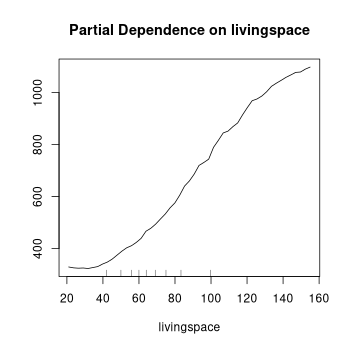
\includegraphics[width=0.6\linewidth]{Partial_Dependence_livingspace.png}\\
        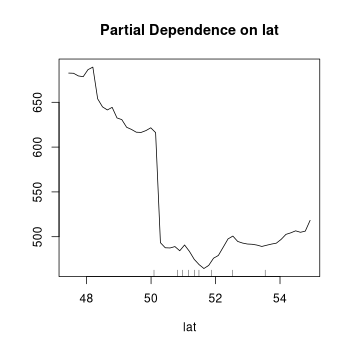
\includegraphics[width=0.6\linewidth]{Partial_Dependence_lat.png}
        \end{figure}
\end{column}
\begin{column}{.5\linewidth}
       \begin{figure}\centering
        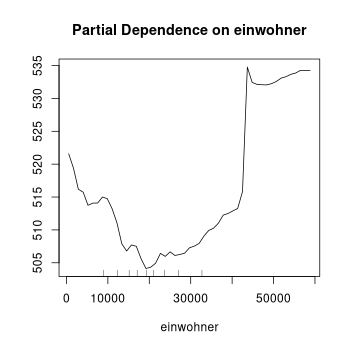
\includegraphics[width=0.6\linewidth]{Partial_Dependence_einwohner.png}\\
        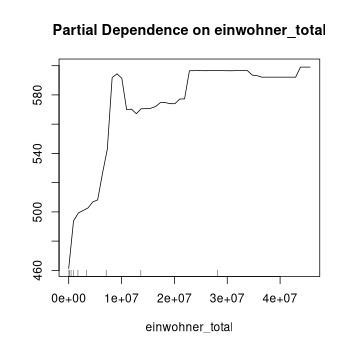
\includegraphics[width=0.6\linewidth]{Partial_Dependence_einwohner_total.png}
       \end{figure}
\end{column}
\end{columns}
\end{frame}

\begin{frame}{Variable Importance}
\end{frame}

\end{document}
